\documentclass[12pt,journal,compsoc]{IEEEtran}
\providecommand{\PSforPDF}[1]{#1}
\hyphenation{op-tical net-works semi-conduc-tor}
\usepackage[font=small,labelfont=bf]{caption}
\usepackage{graphicx}
\usepackage{float}
\floatstyle{boxed}
\restylefloat{figure}

\begin{document}
\title{Evolutionary Design of Flocking Particles for Collectively Intelligent Problem Solving}
\author{Benjamin~Bengfort,~Kevin~Harrison,~and~Philip~Kim}

\IEEEcompsoctitleabstractindextext{%
\begin{abstract}

Self-organizing "flocks" of agents that display emergent coordinated behavior can be implemented using only local interaction rules. When agents are also given memory and a goal-based Finite State Machine (FSM) controller, the resulting team is able to solve a locate-and-collect task. We show that Evolutionary Computing techiques can be applied to the FSM controller, where the genotype is a real valued vector representing the FSM and the phenotype is the emergent, self-organizing behavior. Comparing the resulting FSMs to similar controllers described in the previous literature, we find that the evolved FSMs perform as well as or better than those designed by human  observation. In this paper we will propose methods for applying evolutionary techniques to the structure and states of the controller, perhaps leading to the emergence of novel behavior.

\end{abstract}}

% make the title area
\maketitle

\IEEEdisplaynotcompsoctitleabstractindextext

\section{Introduction}

Ever since Reynolds demonstrated that flocks of birds could be simulated as multi-agent systems \cite{reynolds1987flocks}, wherein each agent's motion is determined solely by local interactions with other agents, there has been interest in extending such systems to solve more general problems. The self-organizing characteristic of these systems, whereby coordinated behavior emerges without a central control mechanism, suggests that even relatively simple decentralized systems might yield novel approaches to problems in both the computational and physical domains.

By abstracting the idea of "flocks" to $n$-dimensional spaces, for example, particle swarms \cite{kennedy1995particle,clerc2002particle} or cultural algorithms \cite{chung1996testbed} have been used for numerical optimization. In the physical domain, swarm behaviors have been used to control multirobot team movement \cite{balch1998behavior,ccelikkanat2010steering,hodgins1994robot}, or during deployment of mobile robots or sensors. In \cite{cheng2009distributed}, flocking behavior was used to maximize area coverage during such deployments coordinating movements via collective behavior. Other tasks using collective problem solving being explored include urban pursuit \cite{winder2004using} and robot herding of animals \cite{vaughan1998robot}.

Many approaches augment the agents with such features as working memory \cite{winder2012role,hu2003particle}. Our paper builds upon the work of Rodriguez \& Reggia in \cite{rodriguez2004extending}, who added both working memory and a finite state machine (FSM) controller that switched the agent between different sets of movement behaviors according to its local environment and current goal. They were able to demonstrate that a team of such agents was able to solve a resource locate-and-collect problem, and that a team programmed with flocking behaviors outperformed teams of agents that did not influence each other's movements.

Attempts have been made to formalize the design of such cooperative multi-agent systems \cite{mataric1993designing,capera2003amas}. In this paper, however, we turn to evolutionary computation techniques. Genetic Programming (GP) \cite{koza1992genetic}, Evolutionary Strategies \cite{rechenberg1989evolution}, and Genetic Algorithms \cite{goldberg1988genetic} have demonstrated the potential of computational design techniques for machine learning, optimization, and even engineering. Swarm techniques have even been applied to evolutionary computation itself as in  \cite{wei2002swarm,miranda2005evolutionary}. However, we are more interested in the opposite application, using evolutionary techniques to determine swarm behavior. Finite state machines have been evolved to solve problems such as automatic target detection \cite{benson2000evolving}. Evolving the high level controllers therefore, seems like an extension of the design of multi-agent problem-solving that is inspired by natural design.

In this paper, we have improved the human design of particles, particularly those described in \cite{rodriguez2004extending} by applying evolutionary techniques to the agent control mechanisms. A formal human design technique determines the structure of the FSM and the parameters defining each state through empirical techniques and inspection. In contrast, we begin with a population of randomly-generated FSM configurations, run them through a simulated problem, then evolve the population over many generations through fitness-based selection, recombination, and mutation. Our hypothesis is that the resulting FSM configuration will perform as well as or better than a configuration tuned by a human.

\section{Methodology}

In order to best demonstrate that an evolutionary process can generate an agent controller that is competitive with a human designed one, we have created an experimental setup that is intentionally similar to the work done in \cite{rodriguez2004extending}. The task is for a team of simulated agents to locate and collect resources that are spread across a large two-dimensional world with periodic boundary conditions, then return the resources to a designated home base.

The individuals of the team operate as a flock- local rules determining individual movement and goals lead to emergent collective behavior. Each individual has a limited sight range and angle, the ability to communicate with other, nearby agents and a limited working memory. Particle behavior is governed by a finite state machine that determines how each particle moves given its individual state and the environment around it.

The task is competitive, as there are two teams in the environment competing for the resources and therefore the simulation is non-deterministic. Agents can mine resources not only from designated depots, but also steal from the home base of the other team. The winner of a simulation is determined as the team that has the most resources in their home base at the end of a predetermined number of time steps.

The evolutionary process uses this simulation to pit individuals created via genetic operations against the best designed human agent. The fitness of the evolved team is a function of the resources that they have collected vs. the resources the other team collected against them. The next generation of evolution is then dependent on the fitness of teams as run in the simulation. In the parlance of evolutionary computing, the genotype is the real valued vector that represents the finite state machine of the particle and the phenotype is the emergent behavior of the team as a whole as it participates in the simulation.

In this section we will present the details of the simulation, as well as the details of the evolutionary computation mechanism that searches for the optimal, most economic particle in the simulation.

\subsection{Simulation}

The movement behavior of individual particles is governed by local interactions of particles within a particlar neighborhood. The particle updates its velocity at each timestep based on what it obeserves in the world around it. This leads to self-organizing, emergent behavior of the flock as a combined whole of its individuals. In particular, movement behaviors are updated with six velocity components: cohesion, alignment, separation, seeking, clearance, and avoidance. Together these components enable flocking behavior, minimize collisions, and strike a balance between the exploration of the world and the exploitation of discovered minerals.

It is important to discuss each individual velocity component in detail, as these components define the movement behaviors of the states that compose the FSM controller that is being evolved. Every component has several parameters: a radius, $r$ and alpha, $\alpha$, which determine the sight distance and angle of the neighborhood of the particular component. Each component additionaly has a weight, $w$, which is used to determine the contribution of the component to the final velocity of the particle.

\subsubsection{Velocity Components}

All particles are bound by a maximum velocity, $v_{max}$ and for the purposes of evolution, a maximum radius, $r_{max}$ to simulate economic constraints in the world. Other notation used is as follows: $\Delta \vec {p} = \vec {p_n} - \vec {p}$ where $\vec {p_n}$ is the average of the neighbor positions and $\vec p$ is the position of the agent. Similarly $\Delta \vec {v} = \vec {v_n} - \vec v$ where $\vec {v_n}$ is the average of the neighbor velocities and $\vec v$ is the velocity of the agent. Other positions include $\vec p_e$ which is the position of an enemy agent and $\vec p_t$, the position of a target and $\vec p_\perp$ represents a unit vector ortogonal to the agent in the $+z$ direction. Specific velocity components are defined as follows.

\textit{Cohesion} (\ref{eqn:cohesion}): a vector pointing towards the average position of friendly agents in the neighborhood, with a magnitude proportional to the agent's distance to the center of its neighbors. This component increases quadratically with distance until it is equal to the maximum velocity when the distance to the neighbor center is $r$. The neighborhood includes all team members who are not guarding or stunned. This velocity component ensures that flocks form and stay together throughout movement.

\begin{equation}
    \vec { v_{ c } } =v_{ max }\frac { \Delta  \vec { p }  }{ \left\|   \Delta \vec { p }  \right\|  } \left( \frac { \left\|  \Delta \vec {  p }  \right\|  }{ r }  \right) ^{ 2 }
    \label{eqn:cohesion}
\end{equation}

\textit{Alignment} (\ref{eqn:alignment}): a vector in the same direction as the average velocity of friendly agents in the neighborhood, with magnitude proportional to the agent's distance to the center of its neighbors. This component increases quadratically with distance until it is equal to the maximum velocity when the distance neighbor center is $r$. The neighborhood includes all team members if they are seeking or spreading. Alignment helps the flock travel in the same direction in a coordinated fashion.

\begin{equation}
    \vec { v_{ al } } =v_{ max }{\left( \frac { \left\| \Delta \vec { p } \right\|  }{ r }  \right)}^2\frac {\Delta \vec{v}} { \left\| \Delta \vec{v} \right\| }
    \label{eqn:alignment}
\end{equation}

\textit{Separation} (\ref{eqn:separation}): a vector pointing away from the average position of friendly agents in the neighborhood, with magnitude inversely proportional to the distance from the agent to the center of its neighbors. This component decreases quadratically with distance until it is zero when the distance to the neighbor center is $r$. The nighborhood includes all team members no matter their state. Separation prevents particles in the same team from colliding with each other, as well as distributing the flock outwards.

\begin{equation}
    \vec { v_{ d } } =-v_{ max }\frac {\Delta \vec{p}} { \left\| \Delta \vec{p} \right\| }{\left( \frac { r - \left\| \Delta \vec { p } \right\|  }{ r }  \right)}^2
    \label{eqn:separation}
\end{equation}

\textit{Seeking, Homing, and Mineral Cohesion} (\ref{eqn:seeking}): vectors pointing directly towards a target with a magnitude proportional to the maximum velocity. These velocity components allow the particle to navigate in a  meaningful manner. The target is stored in memory and this velocity component isn't influenced by nearby neighbors.

\begin{equation}
    \vec{v_h} = v_{max} \frac {\vec{p_t} - \vec p} { \left\| \vec{p_t} - \vec p \right\| }
    \label{eqn:seeking}
\end{equation}

\textit{Clearance} (\ref{eqn:clearance}): a vector pointing in a direction orthogonal to the difference between the average neighbor position and the agent's position proportional the the maximum velocity. This component ensures that swarms have a wide field of view by spreading the flock laterally along the front of movement. The neighborhood of this component is team members in sight that are not guarding or stunned.

\begin{equation}
    \vec{v_{cl}} = v_{max} \frac {\Delta \vec p_\perp } { \left\| \Delta \vec p_\perp  \right\| }
    \label{eqn:clearance}
\end{equation}

\textit{Avoidance} (\ref{eqn:avoidance}): a vector pointing away from an enemy agent in the neighborhood, with magnitude $v_{max}$ when distance to the enemy is zero and decreasing linearly with distance until it is zero when the distance is $r$. Unlike all the other components, this can be applied multiple times each timestep--once for every enemy in the neighborhood.

\begin{equation}
    \vec { v_{ av } } =\sum _{i=0}^{n} {v_{ max } \left( \frac{r - \left\| \Delta \vec{p_e} \right\|} {r} \right) \frac { \Delta \vec { p_e }  }{ \left\| \Delta \vec { p_e }  \right\|  }}
    \label{eqn:avoidance}
\end{equation}

\subsubsection{Movement Behavior}

The FSM controlling each agent in our first experiment contained four states: searching for new resources (SPREADING), moving to the last known resource deposit (SEEKING), carrying resources back to the home location (CARAVANING), or guarding the home base or a resource deposit (GUARDING). Each state was composed of some combination of the previously described velocity components.

To update the velocity of a particle at time $t$, a simple linear combination of velocity components was used. The components, along with their parameters and weights depended on the current state of the particle. The magnitude (or length) of the vector was maximized at $v_{max}$ in the direction of the computed component velocity. Our simulation also implemented "inertia", whereby the velocity was not combined from zero, but rather added to the velocity at time $t-1$. The position of the particle at time $t$ was simply the sum of the position at time $t-1$ with the new velocity.

\begin{equation}
    \vec {v_t} =  \vec {v_{t-1}}+ \sum_i^c { w_i v_i}
    \label{eqn:velocity}
\end{equation}

\begin{equation}
    \vec {p_t} = \vec {p_{t-1}} + \vec {v_t}
    \label{eqn:position}
\end{equation}

Transitions between states were triggered by conditions in each agent's local environment according to rules in the FSM (in our first experiment, these rules were fixed). For example, an agent in the searching state that detected a mineral deposit within a 200-unit radius (in any direction) would push that deposit onto the top of its memory stack and transition to the seeking state (which is characterized by movement toward the top location on its stack).

One of the main findings in \cite{rodriguez2004extending} was that it was advantageous for the agents to post "guards" on their homes and/or on any discovered resource deposits. Agents that guarded only the home performed best of all, though agents that guarded both the home and deposits still outperformed non-guarding agents. In order for guarding behavior to be feasible, however, agents must avoid agents on the enemy team. Since we were allowing evolution to determine the strength of this avoidance parameter, we expected that in the absence of an enforced motivation for avoidance, the avoidance parameter would be selected down to zero, allowing the agents to ignore enemy guards.

Therefore we implemented a penalty for colliding with another agent. An agent within 10 units of an enemy agent was rendered unable to move for a number of timesteps equal to 180 minus the angle of incidence in degrees. For example, if an agent collided with an opposing agent at right angles, the agent struck in the side would be unable to move for 90 timesteps, whereas the agent struck in the front would be unable to move for 180 timesteps. Similarly, being "rear-ended" by an opposing agent had no penalty at all. The hope was that by assigning the "responsible" agent more of the penalty, we would create an incentive to avoid collision.

\begin{figure}[h!]
    \centering
        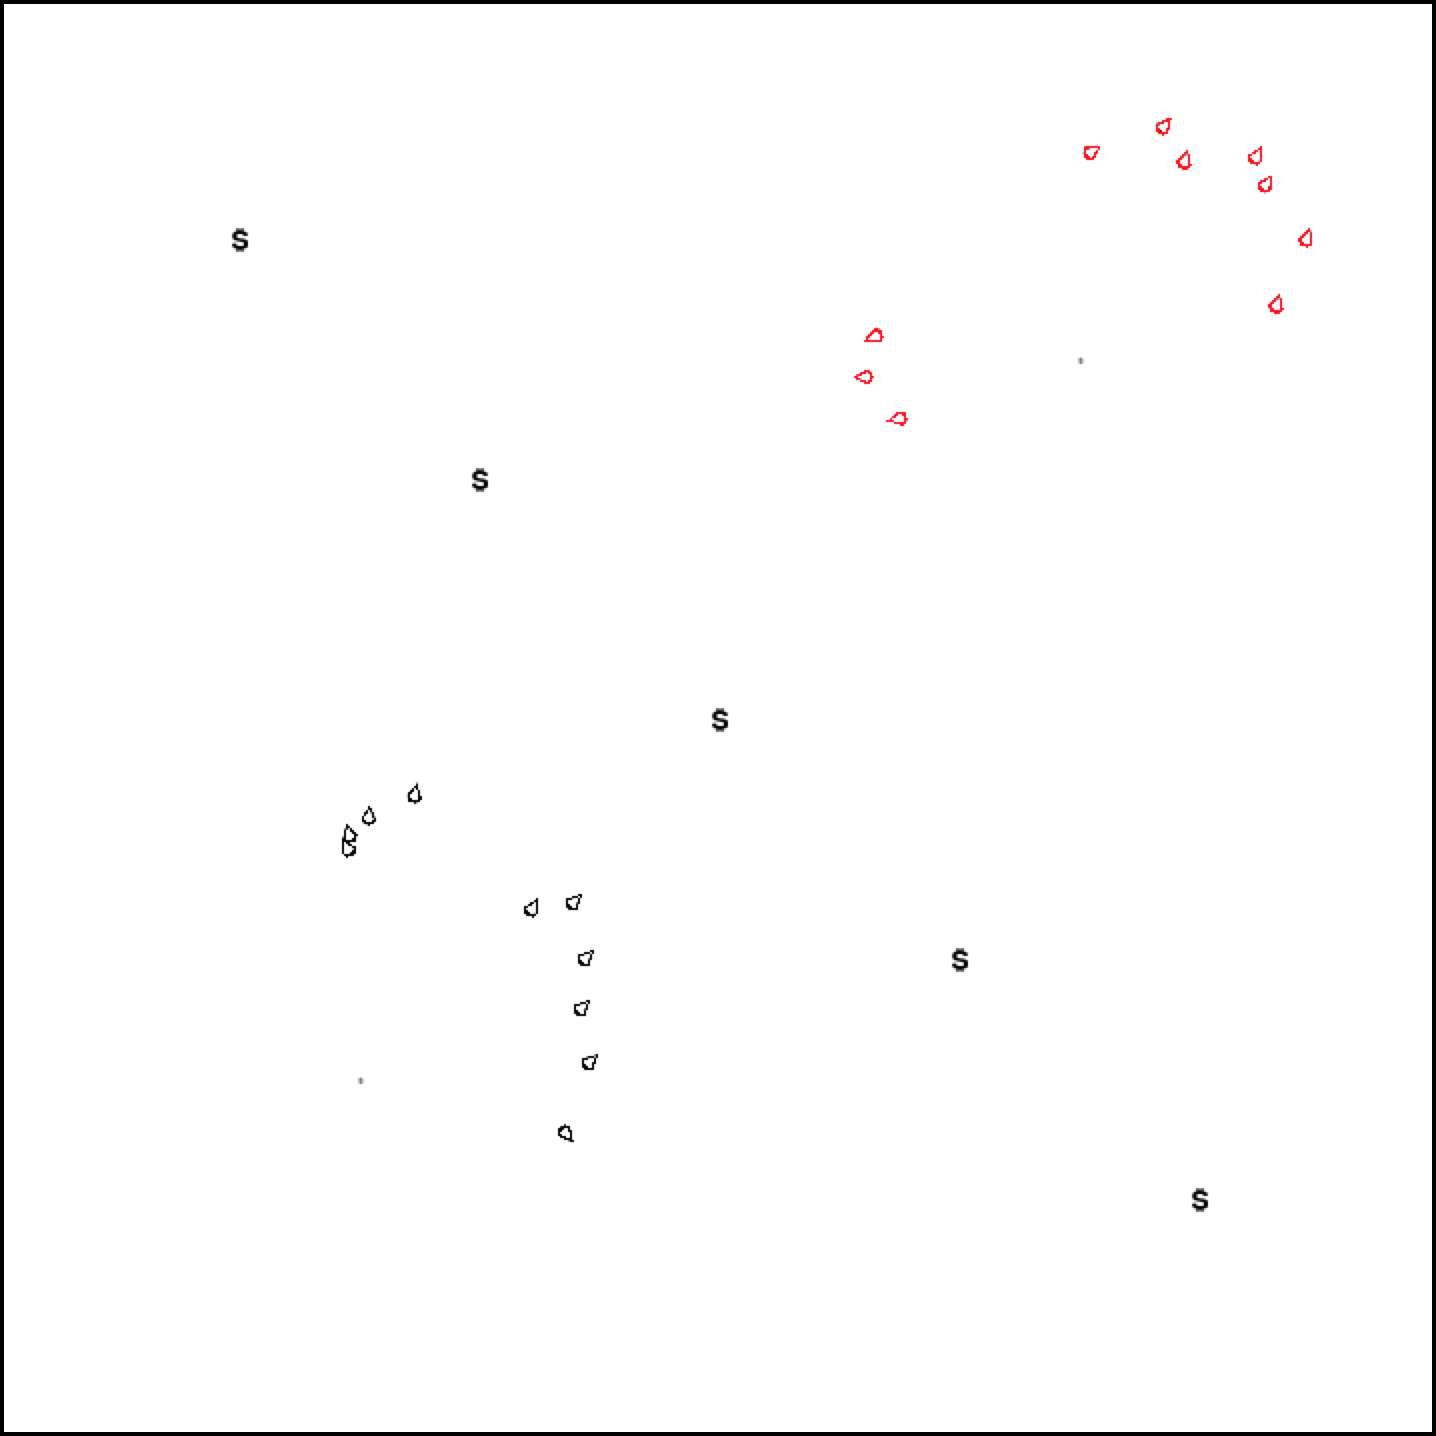
\includegraphics[width=0.5\textwidth]{figures/simulation}
    \caption{Simulation of agents spreading in flocks.}
\end{figure}

In order to allow for the selection of guarding behavior, the transition to the guarding state was controlled by two  evolvable parameters -- the \textit{home guarding threshold} and the \textit{deposit guarding threshold}, which specified the number of friendly agents considered sufficient to guard the respective sites; a value of 0 disabled guarding behavior. This was the only instance in our simulation where a transition between states was controlled by an evolvable parameter, and we will explore adding this component in future work.

A single timestep in the world can be characterized as follows. Each agent is in a particular state. For each velocity component in its current state, it determines the number of friendly and enemy agents in the respective neighborhood and calculates the direction and magnitude of the component. These components are linearly summed, and the resulting velocity is subjected to the $v_{max}$ constraint. The agent's position is updated by adding the velocity to the agent's position in the previous timestep. The agent then determines whether it should change its state based on the predefined transition rules and its current environment. All agents make this computation simultaneously, updating does not affect the world in the current time step.

\subsection{Evolution}

The evolution of a finite state machine for movement control was achieved through the application of a simple set of genetic operators to the states of the FSM as defined by a collection of velocity components and their behavior specific parameters. The genotype for our simulation was represented as a vector containing two integers, one for each guarding threshold, and real-valued numbers consisting of the alpha parameter, radius, and weight given to each component of each compound movement behavior.

In this experiment, the set of states in each controller was fixed to be the same set of compound behaviors as those found in \cite{rodriguez2004extending}, but with parameters derived through evolutionary programming. This allowed for easy comparison with the authoritative, human-derived solution. In addition, the transitions between states were kept the same except for the guarding thresholds, which were evolved. The basic evolutionary computation was a mixture of Evolutionary Strategy and Evolutionary Programming techniques and is characterized in Table \ref{table:evolvemethod}.

The mutation operator first selected which parameters to modify independently. We used a mutation probability parameter $p_m=0.2$  for mutating each weight, radius, alpha, and threshold. Each selected threshold had an equal chance of increasing by 1 and decreasing by 1. Each selected real-valued parameter was modified through the addition of a uniformly distributed random number with mean 0. We mutated each weight with world constraints using $r\in\left(1,500\right]$ and $\alpha\in\left(0,360\right]$, the step size of the mutation was $m_w\in\left[-0.2,0.2\right]$ for weights and $m_s\in\left[20,20\right]$ for the $r$ and $\alpha$ parameters. Elite individuals were exempted from mutation.

The recombination operator also ignored the elite individuals carried over from the last population. Parents were selected with a recombination probability, $p_r=0.2$, to be recombined with another individual. We used intermediary recombination of the weight, radius, and alpha parameters of all components in all states, bounded by the minimum and maximum possible values of each parameter. The second chosen parent remained in the population. Although elite individuals were exempt from recombination, they were able to be selected as the secondary parent, contributing their genetic material to the recombined offspring.

A round of evolution consisted of the evaluation of every individual followed by the application of elitism, tournament selection, recombination, and mutation to produce the next generation. For elitism, the $N_e$ individuals of the previous generation was always carried into the next generation without modification. The other $p-N_e$ individuals were selected via tournaments of size 3. All non-elite individuals chosen through the tournament then each had a $p_r$ chance of undergoing recombination with another randomly chosen child. Each of the resulting non-elite individuals was then subjected to the mutation operator, mutating parameters independently.

\begin{table}
    \renewcommand{\arraystretch}{1.5}
    \centering
    \begin{tabular}{|l|l|}
        \hline
        Genotype & Real valued vectors representing FSM states \\
        Phenotype & Swarm behavior from individual movements \\
        Selection & Tournament with Elitism \\
        Recombination & Intermediary exempting elites \\
        Mutation & Linear Rule exempting elites \\
        Fitness & Resources collected after 10k timesteps \\
        Specialty & Adpating FSM with same size network \\
        \hline
    \end{tabular}
    \caption{Characterization of Evolutionary Method}
    \label{table:evolvemethod}
\end{table}

\section{Experimental Procedure}

Our computational experiment required two main components; a system to carry out the evolutionary computation, which constructed genotype populations via genetic operators, and a simulation system to instantiate phenotypes- particle swarms whose individuals are constructed from the genotypes. The simulation system computed the fitness of a particular swarm, which allowed the evolutionary computation to build the next generation.

The simulation environment consisted of two simulated teams in competition with each other; a red team and a black team. The simulated world was a 3000 x 3000 world with periodic boundary conditions and the number of timesteps was limited to 10,000 per simulation due to computational constraints. We restricted each team to 10 agents each,and evenly distributed 5 resource deposits betwen the red and black bases with 80 resources per deposit. Both the team size and the time limit were implemented to make the evolutionary computation tractable; our implementation required on average 273 seconds to complete; and each generation took approximately 52 minutes to compute all fitness values.

The red team's behavior was implemented using a finite state machine, memory, and movement parameters exactly as the best empirical result designed by humans in \cite{rodriguez2004extending}, called \textit{home guarding flock} meaning that the swarm guarded both its home base but not discovered mineral deposits. The black team utilized the configuration derived from a genotype individual produced by the evolutionary computation. We attempted to hold as many variables constant as possible, including the locations of bases and resources, starting positions and velocities of agents, and update order. After 10,000 timesteps, the fitness of the black team was returned as the number of resources in the black base.

Each simulation was run in parallel as subprocess of a master evolutionary computation process. The master process randomly initialized a population of 50 black team configurations, then ran a simulation for each individual in the population. After all 50 simulations were completed, tournament based selection with tournaments of size three were carried over to the next generation along with the 5 most elite individuals. After selection, genetic operators were applied.

In our first experiment we only used mutation to change the states in the finite state machine of the particles. In the second experiment we used recombination in addition to mutation operations. In either case, elite individuals were exempt from genetic operations, however elite individuals could be recombined to replace other individuals in the population. Both the mutation and recombination (when used) had a likelihood of 0.2. Maximum and minimum parameters were also placed on the values of the weight, the radii, and the alpha values to ensure an economic and reasonable result.

\section{Results}

In this section we will evaluate the effectiveness of both evolved flocking particles vs. human created particles, as well as the ability of an evolutionary computation to design such particles. In short, the evolutionary computation mechanism was able to design a particle system that exhibited variations in behaviors that were different enough from the human designed particles so as not only be competitive with the human design team, but able to defeat the other team in terms of resources collected.

\begin{table}
    \renewcommand{\arraystretch}{1.5}
    \centering
    \begin{tabular}{l | c c cc}
        \hline
        Simulation & Mean & Std Dev & Max & Min \\
        \hline
        human & 119.0 & 43.2 & 274 & 119 \\
        evolved & 296.0 & 25.6 & 336 & 254 \\
        random & 0.3 & 0.67 & 2 & 0 \\
        \hline
    \end{tabular}
    \caption{Aggregated fitness of various particles competing with human designed particles.}
    \label{table:meanfitness}
\end{table}

\begin{figure}[ht!]
    \centering
        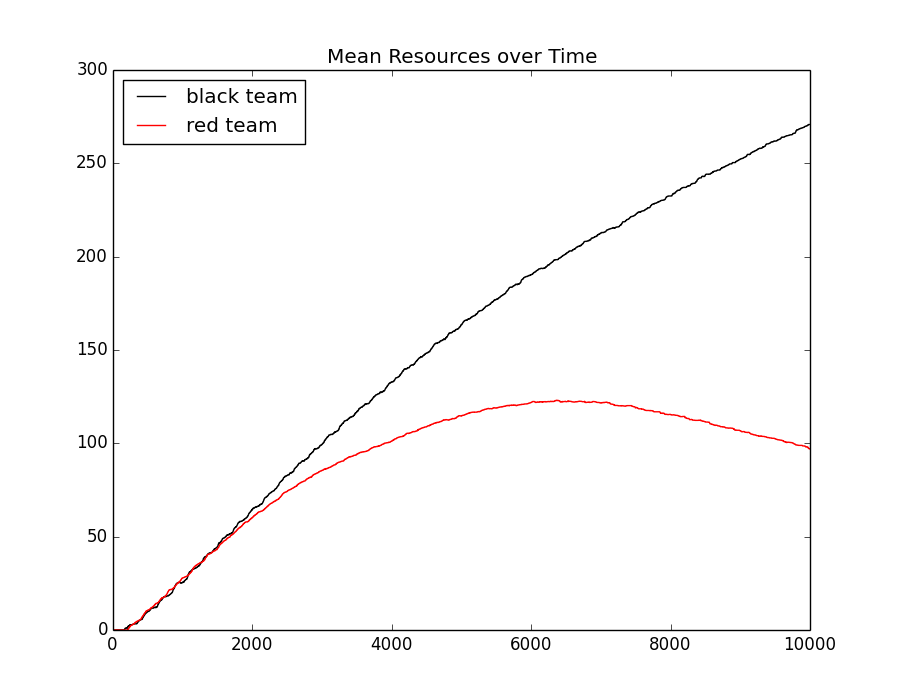
\includegraphics[width=0.5\textwidth]{figures/head2head}
    \caption{Performance of evolved particles vs human designed particles in head to head simulation of 10,000 timesteps}
    \label{fig:head2head}
\end{figure}

Table \ref{table:meanfitness} shows the mean, standard deviation, maximum, and minimum resources collected for the black team over ten runs of the simulation with the same parameters. Black teams of comparsion are the human designed team, the best evolved team, and a random team. The evolution designed team performs significantly better than the human designed team.

The average fitness over time of the black and red teams is displayed in Figure \ref{fig:head2head} which graphs the mean fitness of ten individual runs of the best human designed team (the red team) vs the best evolved team, the black team. Within 6000 timesteps the red team begins to lose resources as the black team exploits the red base in addition to more resource locations than the red team, which favors a strategy of exploiting one resource deposit at a time.

The performance of our two evolutionary computations is expressed in Figures \ref{fig:meanfit1} and \ref{fig:meanfit2} which plots the mean fitness of the entire population per each generation. In experiment one, only the mutation operator was used to generate the next population. In experiment two, both recombination and mutation were used to produce the next generation.

As is shown from the graphs; the first experiment was wildly unstable in terms of its search across the optimal state space. This may have been due to the fact that highly variable mutation caused dramatic shifts in the behavior of the phenotypes. It also may have been due to a programming error on the part of the research team. In the second evolution with recombination as well as mutation, there is more steadily growing fitness over time and a more stable population to select from to apply genetic operations.

\begin{figure}[ht!]
    \centering
        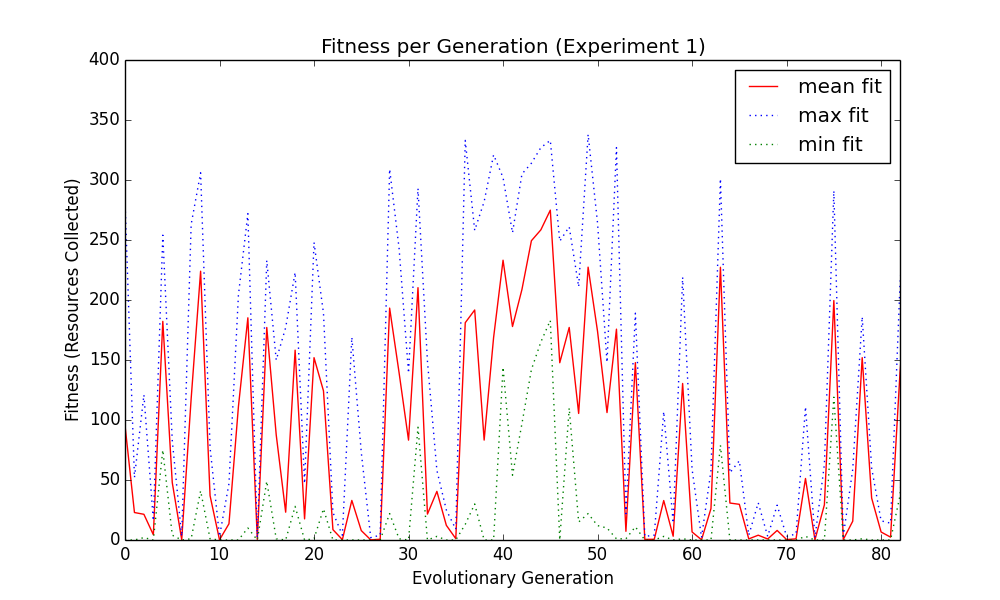
\includegraphics[width=0.5\textwidth]{figures/meanfit_experiment1}
    \caption{Mean fitness per generation with mutation}
    \label{fig:meanfit1}
\end{figure}

\begin{figure}[ht!]
    \centering
        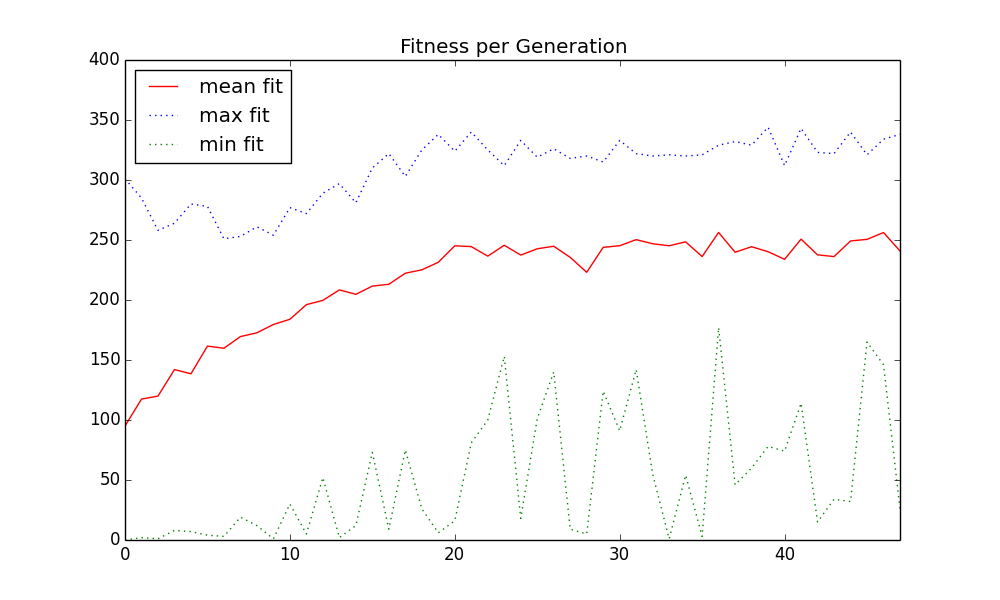
\includegraphics[width=0.5\textwidth]{figures/fitness46}
    \caption{Mean fitness per generation with mutation and recombination}
    \label{fig:meanfit2}
\end{figure}

\section{Discussion}
A nature-inspired, evolutionary technique was successfully able to design particles that not only exhibited collective, emergent behavior, but also surpassed their human design counterparts through a qualitatively novel mechanism. From epirical observation of the best performing teams, it appears that the human designed team prefered to stay in one or two larger flocks; whereas the high performing evolved teams split into more, smaller flocks and were able to exploit the search space more effectively. Because of the limited time frame in the simulation; this was clearly a better strategy, although additional experiments would be needed to determine the success of these particles over a larger time period.

The computational requirements for performing such an evolution were significant particularly in terms of time. However, parallel computation strategies enabled us to gather initial results. Future work might include MapReduce implementations of the evolutionary computation to distribute tasks across a cluster of computers, as well as longer runs to ensure more significant evolutionary behavior. In order to carry out further experimentation at scale, some larger computational framework would be needed to implement the demands of the simulations.

In particular, the work described in this paper represents only the first steps in the application of evolutionary techniques to the design of particles that exhibit flocking behavior. By mutating and applying selective pressure to the movement component parameters, we were able to show that a machine could optimize bottom-up velocity parameters better than a person, along with some limited state transition logic. However, because the states of the FSM controller were encoded in the simulation, we have not shown the ability to generate novel logical behaviors; simply better collective strategies.

The next steps for this research would be to continue to evolve the structure of the FSM in more meaningful ways. In particular, new states should be generated by the configuration of their individual velocity components as well as other evolved conditional rules; not just the state parameters. Of interest is the opportunity to evolve the transitions between states in a more significant manner, and then to go further and evolve the size and structure of the FSM by adding and removing states.

One essential research question that should be answered is whether or not some form of cross-over is possible in the FSM networks of particle swarms. If so, this will open up more opportunties for searching the optimal FSM space for collective movments. Other research questions might include better fitness functions that utilize the state of the entire world (for example, punishing swarms for allowing enemy agents to collect resources), and speciation for different strategies of evolution.

\bibliographystyle{plain}
\bibliography{paper}

\end{document}
